\section{Introduction}


\subsection{What is a decision tree?} \label{whatisadecisiontree}
A business student with only a very few programming skills shall develop a simple algorithm for sorting three elements $A, B, C$. He decides to divide this problem in smaller subproblems. First he wonders if $A$ is smaller then $B$. In the second step it is interesting if $B$ is smaller then $C$. If $A<B$ and $B<C$ then $A<B<C$. But if $B$ is not greater then $C$, then a third question is relevant: Is $A<C$? 

His head is spinning. Maybe solving this problem graphically is a better idea. He draws a node for each question and an edge for each answer. All leafs represent the correct order. Figure \ref{fig:sortingtree} shows the resulting graph:

\begin{figure}[!h]
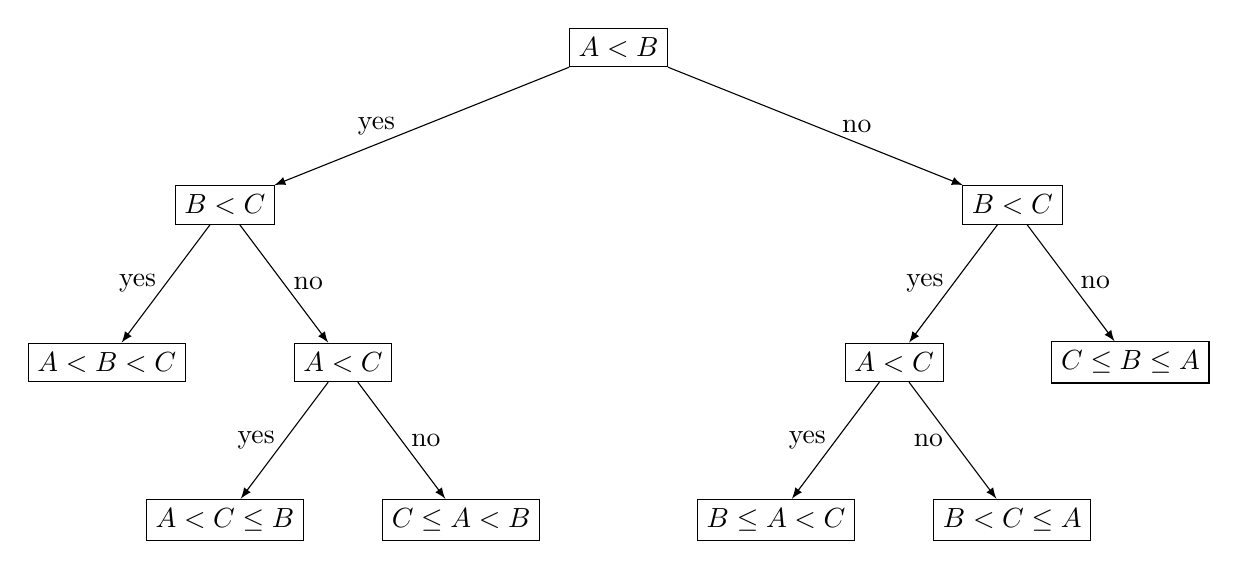
\begin{tikzpicture}[edge from parent/.style={draw,-latex},
level distance=2cm,
level 1/.style={sibling distance=10cm},
level 2/.style={sibling distance=3cm}]
\tikzstyle{every node}=[rectangle,draw]    
\node (Root) {$A < B$}
child {
    node {$B < C$}    
    child { 
        node {$A < B < C$} 
        edge from parent node[left,draw=none] {yes}
    }
    child { 
        node {$A < C$} 
        child {
            node {$A < C \leq B$}
            edge from parent node[left,draw=none] {yes}
        }
        child {
            node {$C \leq A < B$}
            edge from parent node[right,draw=none] {no}
        }
        edge from parent node[right,draw=none] {no}
    }
    edge from parent node[left,draw=none] {yes $\;$}
}
child {
    node {$B < C$}
    child { 
        node {$A < C$}     
        child {
            node {$B \leq A < C$}
            edge from parent node[left,draw=none] {yes}
        }   
        child {
            node {$B < C \leq A$}
            edge from parent node[left,draw=none] {no}
        }     
        edge from parent node[left,draw=none] {yes}
    }
    child { 
        node {$C \leq B \leq A$} 
        edge from parent node[right,draw=none] {no}
    }
    edge from parent node[right,draw=none] { $\;$ no}
};
\end{tikzpicture}
\caption{A decision tree for sorting three values.}
\label{fig:sortingtree}
\end{figure}

Without further knowledge the student created his first decision tree.

For a right decision two or three if-statements are necessary. So a Python program could look like listing \ref{lst:sort1}.

\newpage

\begin{lstlisting}[style = fau, language = Python, caption={[A Python implementation of a decision tree for sorting three elements]A Python implementation of a decision tree for sorting three elements $A, B, C$},label=lst:sort1]
def sort1(A, B, C):
	if (A < B):
		if (B < C):
			return [A, B, C]
		else:
			if (A < C):
				return [A, C, B]
			else:
				return [C, A, B]
	else:
		if (B < C):
			if (A < C):
				return [B, A, C]
			else:
				return [B, C, A]
		else:
			return [C, B, A]

print( sort1(9,-2,0) ) # >> [-2, 0, 9]
print( sort1(2,0,0) )  # >> [0, 0, 2]
\end{lstlisting}

\begin{remark}
    The Python if-statement syntax implies the tree structure in a vertical form, too.      
\end{remark}

Another way of formatting if-clauses represents a rule set which are first order logical expressions:  
    \begin{lstlisting}[style = fau, language = Python, caption={A Python reimplementation of the decision tree given in listing \ref{lst:sort1} as a set of first order logical rules},label=lst:sort2]
def sort2(A, B, C):
	if (A < B) and (B < C) : return [A, B, C]
	if (A < B) and not (B < C) and (A < C): return [A, C, B]
	if (A < B) and not (B < C) and not (A < C): return [C, A, B]
	if not (A < B) and (B < C) and (A < C): return [B, A, C]
	if not (A < B) and (B < C) and not (A < C): return [B, C, A]
	if not (A < B) and not (B < C) : return [C, B, A]
\end{lstlisting}

Unsurprisingly, we get six rules for $3! = 6$ different combinations and the same results as in the algorithm \texttt{sort1}. 


This introductory example shows four important properties: Decision trees
\begin{enumerate}
    \item work very well for classification and data mining.
    \item are intuitive and self-explanatory.
    \item are easy to implement.
    \item can be even used by business students.
\end{enumerate}

\begin{remark}
    Decision trees are used to model all comparison sorts like mergesort or quicksort. The reader may notice that the decision tree in figure \ref{fig:sortingtree} represents the insertion sort algorithm \cite[p. 208]{cormen2001introduction}. 
\end{remark}



